% \documentclass[9pt,t]{beamer}
\usefonttheme{professionalfonts}
\usefonttheme{serif}
\PassOptionsToPackage{pdfpagemode=FullScreen}{hyperref}
\PassOptionsToPackage{usenames,dvipsnames}{color}
% \DeclareGraphicsRule{*}{mps}{*}{}
\usepackage{linalgjh}
\usepackage{present}
\usepackage{directories}  % Define \mapdir, \mapmpdir, etc.
\usepackage{xr}\externaldocument{\mapdir map2} % read refs from .aux file
\usepackage{xr}\externaldocument{\vsdir vs3} % read refs from .aux file
\usepackage{catchfilebetweentags}
\usepackage{etoolbox} % from http://tex.stackexchange.com/questions/40699/input-only-part-of-a-file-using-catchfilebetweentags-package
\makeatletter
\patchcmd{\CatchFBT@Fin@l}{\endlinechar\m@ne}{}
  {}{\typeout{Unsuccessful patch!}}
\makeatother

\mode<presentation>
{
  \usetheme{boxes}
  \setbeamercovered{invisible}
  \setbeamertemplate{navigation symbols}{} 
}
\addheadbox{filler}{\ }  % create extra space at top of slide 
\hypersetup{colorlinks=true,linkcolor=blue} 

\title[Plane transformations] % (optional, use only with long paper titles)
{The action of plane transformations}

\author{\textit{Linear Algebra} \\ {\small Jim Hef{}feron}}
\institute{
  \texttt{http://joshua.smcvt.edu/linearalgebra}
}
\date{}


\subject{Plane transformations}
% This is only inserted into the PDF information catalog. Can be left
% out. 

\begin{document}
\begin{frame}
  \titlepage
\end{frame}

% =============================================
% \begin{frame}{Reduced Echelon Form} 
% \end{frame}



% ..... Three.II.1 .....
\section{Transformations of $\Re^2$}
%..........
\begin{frame}{Lines go to lines}
In a real space $\Re^n$ a line through the origin is a set 
$\set{r\cdot \vec{v}\suchthat r\in\Re}$ of multiples of a 
nonzero vector. 

Consider a transformation
$\map{t}{\Re^n}{\Re^n}$.
% A defining property of linear maps is that 
% $t(r\cdot\vec{v})=r\cdot t(\vec{v})$.
It is linear and so $t$'s action 
\begin{equation*}
  r\cdot\vec{v}\mapsunder{t} r\cdot t(\vec{v})
\end{equation*}
sends members of the line $\set{r\cdot \vec{v}\suchthat r\in\Re}$
in the domain to members of the line
$\set{s\cdot t(\vec{v})\suchthat s\in\Re}$
in the codomain. 

Thus, under a transformation, lines through the origin 
map to lines through the origin.
Further, the action of~$t$ is determined by its effect $t(\vec{v})$
on any nonzero element of the domain line.
\end{frame}
\begin{frame}
\ex
Consider the line~$y=2x$ in the plane 
\begin{equation*}
  \set{r\cdot\colvec{1 \\ 2}\suchthat r\in\Re}
\end{equation*}
and this transformation.
\begin{equation*}
  \colvec{x \\ y}
  \mapsto
  \colvec{x+3y \\ 2x+4y}
\end{equation*}
The map's effect on any vector in the line is easy to compute.
\begin{equation*}
  \vec{v}=\colvec{1 \\ 2}\mapsunder{t}\colvec{7 \\ 10}
\end{equation*}
The linear map property 
$t(r\cdot\vec{v})=r\cdot t(\vec{v})$
imposes a uniformity on $t$'s action:~$t$ 
has twice the effect on $2\vec{v}$, three times the
effect on $3\vec{v}$, etc.
\begin{equation*}
  \colvec{2 \\ 4}\mapsunder{t}\colvec{14 \\ 20}
  \qquad
  \colvec{-3 \\ -6}\mapsunder{t}\colvec{-21 \\ -30}
  \qquad
  \colvec{r \\ 2r}\mapsunder{t}\colvec{7r \\ 10r}
\end{equation*}
In short: the action of $t$ on any  nonzero $\vec{v}$
determines its action on any other vector $r\vec{v}$
in the line $\spanof{\vec{v}}$.
\end{frame}


\begin{frame}
  \frametitle{Pick one, any one}
Every plane vector is in some line through the origin
so to understand what $\map{t}{\Re^2}{\Re^2}$ does 
to plane elements it suffices to 
understand what it does to lines through the origin. 
\pause
By the prior slide, to understand what $t$ does to a line through the 
origin it suffices to understand what it does to a single nonzero
vector in that line.

\pause
So one way to understand a transformation's action is to take
a set containing one nonzero vector from each line through the origin,
and describe where the transformation maps the elements of that set.

A natural set with one nonzero element from each line through the
origin is the upper half unit circle (we will explain the colors below).
\begin{equation*}
  \set{\colvec{x \\ y}
       =\colvec{\cos(t) \\ \sin(t)}
         \suchthat 
         0\leq t<\pi}
  \qquad
  \vcenteredhbox{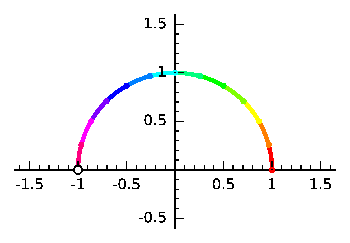
\includegraphics[scale=.75]{graphics/three_ii_a_unithalfcircle.pdf}}  
\end{equation*}  
\end{frame}


\begin{frame}{Dilate $x$}
\ex
The map
\begin{equation*}
  \colvec{x \\ y} \mapsto \colvec{2x \\ y}
\end{equation*}
doubles the first coordinate while keeping the second coordinate constant.
This shows the transformation of the upper half circle.
\begin{equation*}
  \vcenteredhbox{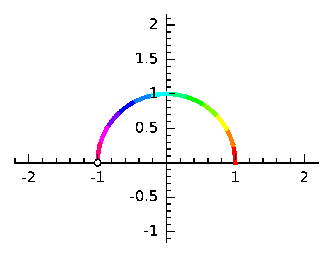
\includegraphics[scale=.75]{graphics/three_ii_a_dialatex1.pdf}}
  \quad\rightarrow\quad
  \vcenteredhbox{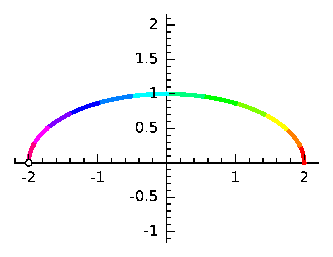
\includegraphics[scale=.75]{graphics/three_ii_a_dialatex2.pdf}}
\end{equation*}
\end{frame}


\begin{frame}{Reverse orientation}
\ex
Here we dilate by a negative.
\begin{equation*}
  \colvec{x \\ y} \mapsto \colvec{-x \\ y}
\end{equation*}
The transformation of the upper half circle
shows why we used the colors.
In the domain they are, taken counterclockwise, red, orange, yellow,
green, blue, indigo, violet.
In the codomain, again taken counterclockwise, they do the opposite. 
\begin{equation*}
  \vcenteredhbox{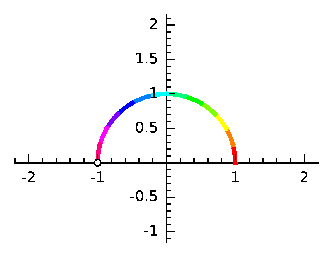
\includegraphics[scale=.75]{graphics/three_ii_a_reversex1.pdf}}
  \quad\rightarrow\quad
  \vcenteredhbox{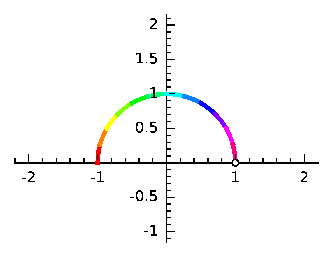
\includegraphics[scale=.75]{graphics/three_ii_a_reversex2.pdf}}
\end{equation*}
\end{frame}


\begin{frame}{Combine dilations}
\ex
Here we dilate both $x$ and~$y$.
\begin{equation*}
  \colvec{x \\ y} \mapsto \colvec{-x \\ 3y}
\end{equation*}
Again the color order reverses, in addition to the stretching 
along the $y$~axis.
\begin{equation*}
  \vcenteredhbox{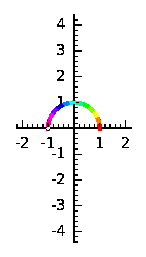
\includegraphics[scale=.75]{graphics/three_ii_a_diagmap1.pdf}}
  \quad\rightarrow\quad
  \vcenteredhbox{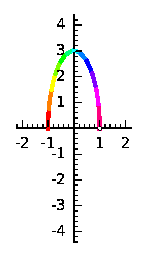
\includegraphics[scale=.75]{graphics/three_ii_a_diagmap2.pdf}}
\end{equation*}
The two dilations 
combine independently in that the first coordinate of the output uses 
only~$x$ and the second coordinate of the output uses only~$y$. 
\end{frame}


\begin{frame}{Skew}
\ex
Next is a map with an output coordinate affected by both $x$ and~$y$.
\begin{equation*}
  \colvec{x \\ y} \mapsto \colvec{x+2y \\ y}
\end{equation*}
\begin{equation*}
  \vcenteredhbox{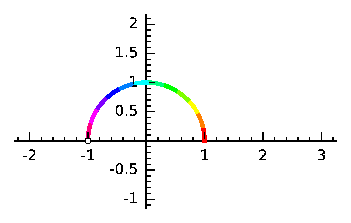
\includegraphics[scale=.75]{graphics/three_ii_a_skew1.pdf}}
  \quad\rightarrow\quad
  \vcenteredhbox{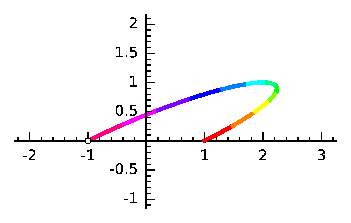
\includegraphics[scale=.75]{graphics/three_ii_a_skew2.pdf}}
\end{equation*}
On the $x$~axis, where~$y=0$, the output's first coordinate is the 
same as the input's first coordinate.
However as we move away from the $x$~axis the $y$'s get larger, and the 
first coordinate of the output is increasingly affected.
(One definition of \textit{skew} is:~having an oblique direction or 
position; slanting.)
\end{frame}


\begin{frame}{Skew the other way}
\ex
We can flip which output coordinate is affected by both $x$ and~$y$.
\begin{equation*}
  \colvec{x \\ y} \mapsto \colvec{x \\ 2x+y}
\end{equation*}
\begin{equation*}
  \vcenteredhbox{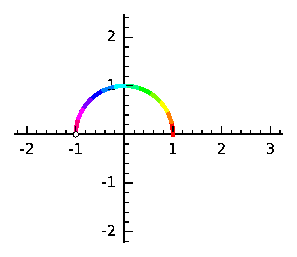
\includegraphics[scale=.75]{graphics/three_ii_a_changeskew1.pdf}}
  \quad\rightarrow\quad
  \vcenteredhbox{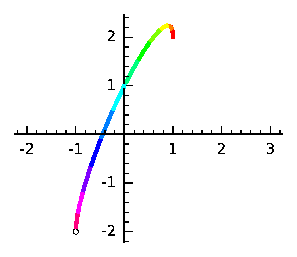
\includegraphics[scale=.75]{graphics/three_ii_a_changeskew2.pdf}}
\end{equation*}
In addition to dilation 
we see clear rotation, for instance of 
the red input vector. 
\end{frame}


\begin{frame}{Same idea but with a smaller effect}
\ex
\begin{equation*}
  \colvec{x \\ y} \mapsto \colvec{x \\ (1/2)x+y}
\end{equation*}
\begin{equation*}
  \vcenteredhbox{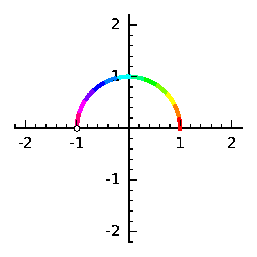
\includegraphics[scale=.75]{graphics/three_ii_a_otherskew1.pdf}}
  \quad\rightarrow\quad
  \vcenteredhbox{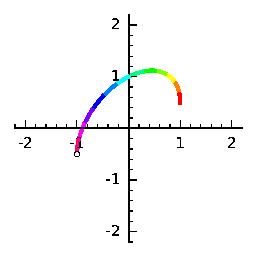
\includegraphics[scale=.75]{graphics/three_ii_a_otherskew2.pdf}}
\end{equation*}
Observe that the rotation is not even.  
A red vector is rotated quite a bit but a green vector, near the
$y$~axis, is not rotated much.
And right on the $y$-axis the vector is not rotated at all. 
\end{frame}


\begin{frame}{Pure roation}
\ex
This rotates every vector counterclockwise through the angle~$\theta$. 
\begin{equation*} 
  \colvec{x \\ y} \mapsto \colvec{\cos(\theta)\cdot x-\sin(\theta)\cdot y \\ \cos(\theta)\cdot x+\sin(\theta)\cdot y} 
\end{equation*}
In this picture $\theta=\pi/6$.
\begin{equation*}
  \vcenteredhbox{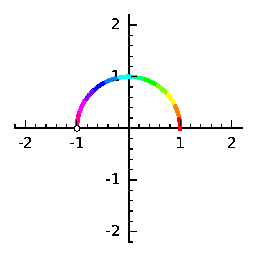
\includegraphics[scale=.75]{graphics/three_ii_a_rotation1.pdf}}
  \quad\rightarrow\quad
  \vcenteredhbox{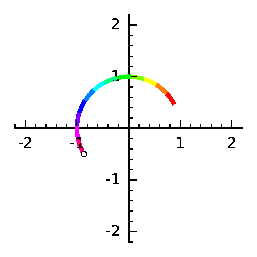
\includegraphics[scale=.75]{graphics/three_ii_a_rotation2.pdf}}
\end{equation*}
\end{frame}


\begin{frame}{Projection}
\ex
Maps can lose a dimension. 
\begin{equation*} 
  \colvec{x \\ y} \mapsto \colvec{x \\ 0}
\end{equation*}
The output is one-dimensional.
\begin{equation*}
  \vcenteredhbox{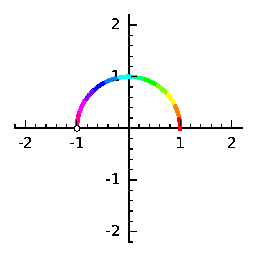
\includegraphics[scale=.75]{graphics/three_ii_a_projection1.pdf}}
  \quad\rightarrow\quad
  \vcenteredhbox{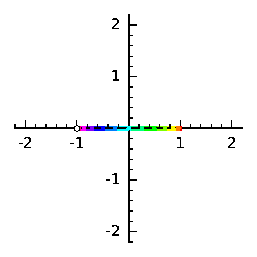
\includegraphics[scale=.75]{graphics/three_ii_a_projection2.pdf}}
\end{equation*}
\end{frame}


\begin{frame}
\ex
The map may project the input vector to a line that is not an axis.
\begin{equation*} 
  \colvec{x \\ y} \mapsto \colvec{x \\ 2x}
\end{equation*}
The two-dimensional input is sent to an output that is one-dimensional.
\begin{equation*}
  \vcenteredhbox{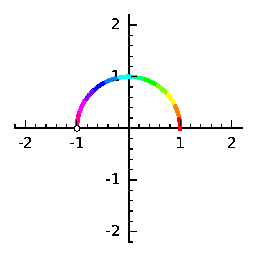
\includegraphics[scale=.75]{graphics/three_ii_a_otherprojection1.pdf}}
  \quad\rightarrow\quad
  \vcenteredhbox{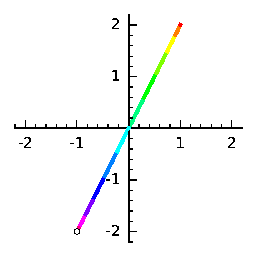
\includegraphics[scale=.75]{graphics/three_ii_a_otherprojection2.pdf}}
\end{equation*}
\end{frame}


\begin{frame}{A generic map}
\ex
An arbitrary map 
\begin{equation*} 
  \colvec{x \\ y} \mapsto \colvec{x+2y \\ 3x+4y}
\end{equation*}
may have an action that is a mixture of the effects shown above.
\begin{equation*}
  \vcenteredhbox{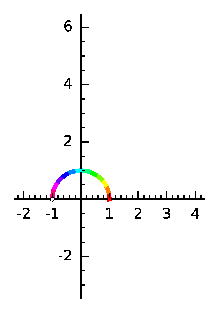
\includegraphics[scale=.75]{graphics/three_ii_a_generic1.pdf}}
  \quad\rightarrow\quad
  \vcenteredhbox{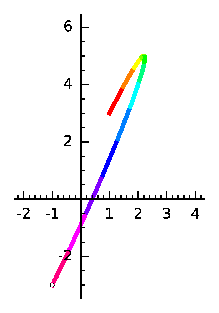
\includegraphics[scale=.75]{graphics/three_ii_a_generic2.pdf}}
\end{equation*}
This shows dilation, rotation, and orientation reversal.
\end{frame}





%...........................
% \begin{frame}
% \ExecuteMetaData[../gr3.tex]{GaussJordanReduction}
% \df[def:RedEchForm]
% 
% \end{frame}
\end{document}
